\documentclass[letterpaper,compsoc,twoside]{IEEEtran}
% generated by Docutils <http://docutils.sourceforge.net/>
\usepackage{cmap} % fix search and cut-and-paste in Acrobat
\usepackage{ifthen}
\usepackage[T1]{fontenc}
\usepackage[utf8]{inputenc}
\usepackage{amsmath}
\usepackage{booktabs}
\usepackage{color}

\usepackage[font={small,it},labelfont=bf]{caption}
\usepackage{float}


\setcounter{secnumdepth}{0}
\usepackage{longtable,ltcaption,array}
\setlength{\extrarowheight}{2pt}
\newlength{\DUtablewidth} % internal use in tables

%%% Custom LaTeX preamble
\usepackage{scipy}
\makeatletter
\def\PY@reset{\let\PY@it=\relax \let\PY@bf=\relax%
    \let\PY@ul=\relax \let\PY@tc=\relax%
    \let\PY@bc=\relax \let\PY@ff=\relax}
\def\PY@tok#1{\csname PY@tok@#1\endcsname}
\def\PY@toks#1+{\ifx\relax#1\empty\else%
    \PY@tok{#1}\expandafter\PY@toks\fi}
\def\PY@do#1{\PY@bc{\PY@tc{\PY@ul{%
    \PY@it{\PY@bf{\PY@ff{#1}}}}}}}
\def\PY#1#2{\PY@reset\PY@toks#1+\relax+\PY@do{#2}}

\expandafter\def\csname PY@tok@w\endcsname{\def\PY@tc##1{\textcolor[rgb]{0.73,0.73,0.73}{##1}}}
\expandafter\def\csname PY@tok@c\endcsname{\let\PY@it=\textit\def\PY@tc##1{\textcolor[rgb]{0.25,0.50,0.56}{##1}}}
\expandafter\def\csname PY@tok@cp\endcsname{\def\PY@tc##1{\textcolor[rgb]{0.00,0.44,0.13}{##1}}}
\expandafter\def\csname PY@tok@cs\endcsname{\def\PY@tc##1{\textcolor[rgb]{0.25,0.50,0.56}{##1}}\def\PY@bc##1{\setlength{\fboxsep}{0pt}\colorbox[rgb]{1.00,0.94,0.94}{\strut ##1}}}
\expandafter\def\csname PY@tok@k\endcsname{\let\PY@bf=\textbf\def\PY@tc##1{\textcolor[rgb]{0.00,0.44,0.13}{##1}}}
\expandafter\def\csname PY@tok@kp\endcsname{\def\PY@tc##1{\textcolor[rgb]{0.00,0.44,0.13}{##1}}}
\expandafter\def\csname PY@tok@kt\endcsname{\def\PY@tc##1{\textcolor[rgb]{0.56,0.13,0.00}{##1}}}
\expandafter\def\csname PY@tok@o\endcsname{\def\PY@tc##1{\textcolor[rgb]{0.40,0.40,0.40}{##1}}}
\expandafter\def\csname PY@tok@ow\endcsname{\let\PY@bf=\textbf\def\PY@tc##1{\textcolor[rgb]{0.00,0.44,0.13}{##1}}}
\expandafter\def\csname PY@tok@nb\endcsname{\def\PY@tc##1{\textcolor[rgb]{0.00,0.44,0.13}{##1}}}
\expandafter\def\csname PY@tok@nf\endcsname{\def\PY@tc##1{\textcolor[rgb]{0.02,0.16,0.49}{##1}}}
\expandafter\def\csname PY@tok@nc\endcsname{\let\PY@bf=\textbf\def\PY@tc##1{\textcolor[rgb]{0.05,0.52,0.71}{##1}}}
\expandafter\def\csname PY@tok@nn\endcsname{\let\PY@bf=\textbf\def\PY@tc##1{\textcolor[rgb]{0.05,0.52,0.71}{##1}}}
\expandafter\def\csname PY@tok@ne\endcsname{\def\PY@tc##1{\textcolor[rgb]{0.00,0.44,0.13}{##1}}}
\expandafter\def\csname PY@tok@nv\endcsname{\def\PY@tc##1{\textcolor[rgb]{0.73,0.38,0.84}{##1}}}
\expandafter\def\csname PY@tok@no\endcsname{\def\PY@tc##1{\textcolor[rgb]{0.38,0.68,0.84}{##1}}}
\expandafter\def\csname PY@tok@nl\endcsname{\let\PY@bf=\textbf\def\PY@tc##1{\textcolor[rgb]{0.00,0.13,0.44}{##1}}}
\expandafter\def\csname PY@tok@ni\endcsname{\let\PY@bf=\textbf\def\PY@tc##1{\textcolor[rgb]{0.84,0.33,0.22}{##1}}}
\expandafter\def\csname PY@tok@na\endcsname{\def\PY@tc##1{\textcolor[rgb]{0.25,0.44,0.63}{##1}}}
\expandafter\def\csname PY@tok@nt\endcsname{\let\PY@bf=\textbf\def\PY@tc##1{\textcolor[rgb]{0.02,0.16,0.45}{##1}}}
\expandafter\def\csname PY@tok@nd\endcsname{\let\PY@bf=\textbf\def\PY@tc##1{\textcolor[rgb]{0.33,0.33,0.33}{##1}}}
\expandafter\def\csname PY@tok@s\endcsname{\def\PY@tc##1{\textcolor[rgb]{0.25,0.44,0.63}{##1}}}
\expandafter\def\csname PY@tok@sd\endcsname{\let\PY@it=\textit\def\PY@tc##1{\textcolor[rgb]{0.25,0.44,0.63}{##1}}}
\expandafter\def\csname PY@tok@si\endcsname{\let\PY@it=\textit\def\PY@tc##1{\textcolor[rgb]{0.44,0.63,0.82}{##1}}}
\expandafter\def\csname PY@tok@se\endcsname{\let\PY@bf=\textbf\def\PY@tc##1{\textcolor[rgb]{0.25,0.44,0.63}{##1}}}
\expandafter\def\csname PY@tok@sr\endcsname{\def\PY@tc##1{\textcolor[rgb]{0.14,0.33,0.53}{##1}}}
\expandafter\def\csname PY@tok@ss\endcsname{\def\PY@tc##1{\textcolor[rgb]{0.32,0.47,0.09}{##1}}}
\expandafter\def\csname PY@tok@sx\endcsname{\def\PY@tc##1{\textcolor[rgb]{0.78,0.36,0.04}{##1}}}
\expandafter\def\csname PY@tok@m\endcsname{\def\PY@tc##1{\textcolor[rgb]{0.13,0.50,0.31}{##1}}}
\expandafter\def\csname PY@tok@gh\endcsname{\let\PY@bf=\textbf\def\PY@tc##1{\textcolor[rgb]{0.00,0.00,0.50}{##1}}}
\expandafter\def\csname PY@tok@gu\endcsname{\let\PY@bf=\textbf\def\PY@tc##1{\textcolor[rgb]{0.50,0.00,0.50}{##1}}}
\expandafter\def\csname PY@tok@gd\endcsname{\def\PY@tc##1{\textcolor[rgb]{0.63,0.00,0.00}{##1}}}
\expandafter\def\csname PY@tok@gi\endcsname{\def\PY@tc##1{\textcolor[rgb]{0.00,0.63,0.00}{##1}}}
\expandafter\def\csname PY@tok@gr\endcsname{\def\PY@tc##1{\textcolor[rgb]{1.00,0.00,0.00}{##1}}}
\expandafter\def\csname PY@tok@ge\endcsname{\let\PY@it=\textit}
\expandafter\def\csname PY@tok@gs\endcsname{\let\PY@bf=\textbf}
\expandafter\def\csname PY@tok@gp\endcsname{\let\PY@bf=\textbf\def\PY@tc##1{\textcolor[rgb]{0.78,0.36,0.04}{##1}}}
\expandafter\def\csname PY@tok@go\endcsname{\def\PY@tc##1{\textcolor[rgb]{0.20,0.20,0.20}{##1}}}
\expandafter\def\csname PY@tok@gt\endcsname{\def\PY@tc##1{\textcolor[rgb]{0.00,0.27,0.87}{##1}}}
\expandafter\def\csname PY@tok@err\endcsname{\def\PY@bc##1{\setlength{\fboxsep}{0pt}\fcolorbox[rgb]{1.00,0.00,0.00}{1,1,1}{\strut ##1}}}
\expandafter\def\csname PY@tok@kc\endcsname{\let\PY@bf=\textbf\def\PY@tc##1{\textcolor[rgb]{0.00,0.44,0.13}{##1}}}
\expandafter\def\csname PY@tok@kd\endcsname{\let\PY@bf=\textbf\def\PY@tc##1{\textcolor[rgb]{0.00,0.44,0.13}{##1}}}
\expandafter\def\csname PY@tok@kn\endcsname{\let\PY@bf=\textbf\def\PY@tc##1{\textcolor[rgb]{0.00,0.44,0.13}{##1}}}
\expandafter\def\csname PY@tok@kr\endcsname{\let\PY@bf=\textbf\def\PY@tc##1{\textcolor[rgb]{0.00,0.44,0.13}{##1}}}
\expandafter\def\csname PY@tok@bp\endcsname{\def\PY@tc##1{\textcolor[rgb]{0.00,0.44,0.13}{##1}}}
\expandafter\def\csname PY@tok@fm\endcsname{\def\PY@tc##1{\textcolor[rgb]{0.02,0.16,0.49}{##1}}}
\expandafter\def\csname PY@tok@vc\endcsname{\def\PY@tc##1{\textcolor[rgb]{0.73,0.38,0.84}{##1}}}
\expandafter\def\csname PY@tok@vg\endcsname{\def\PY@tc##1{\textcolor[rgb]{0.73,0.38,0.84}{##1}}}
\expandafter\def\csname PY@tok@vi\endcsname{\def\PY@tc##1{\textcolor[rgb]{0.73,0.38,0.84}{##1}}}
\expandafter\def\csname PY@tok@vm\endcsname{\def\PY@tc##1{\textcolor[rgb]{0.73,0.38,0.84}{##1}}}
\expandafter\def\csname PY@tok@sa\endcsname{\def\PY@tc##1{\textcolor[rgb]{0.25,0.44,0.63}{##1}}}
\expandafter\def\csname PY@tok@sb\endcsname{\def\PY@tc##1{\textcolor[rgb]{0.25,0.44,0.63}{##1}}}
\expandafter\def\csname PY@tok@sc\endcsname{\def\PY@tc##1{\textcolor[rgb]{0.25,0.44,0.63}{##1}}}
\expandafter\def\csname PY@tok@dl\endcsname{\def\PY@tc##1{\textcolor[rgb]{0.25,0.44,0.63}{##1}}}
\expandafter\def\csname PY@tok@s2\endcsname{\def\PY@tc##1{\textcolor[rgb]{0.25,0.44,0.63}{##1}}}
\expandafter\def\csname PY@tok@sh\endcsname{\def\PY@tc##1{\textcolor[rgb]{0.25,0.44,0.63}{##1}}}
\expandafter\def\csname PY@tok@s1\endcsname{\def\PY@tc##1{\textcolor[rgb]{0.25,0.44,0.63}{##1}}}
\expandafter\def\csname PY@tok@mb\endcsname{\def\PY@tc##1{\textcolor[rgb]{0.13,0.50,0.31}{##1}}}
\expandafter\def\csname PY@tok@mf\endcsname{\def\PY@tc##1{\textcolor[rgb]{0.13,0.50,0.31}{##1}}}
\expandafter\def\csname PY@tok@mh\endcsname{\def\PY@tc##1{\textcolor[rgb]{0.13,0.50,0.31}{##1}}}
\expandafter\def\csname PY@tok@mi\endcsname{\def\PY@tc##1{\textcolor[rgb]{0.13,0.50,0.31}{##1}}}
\expandafter\def\csname PY@tok@il\endcsname{\def\PY@tc##1{\textcolor[rgb]{0.13,0.50,0.31}{##1}}}
\expandafter\def\csname PY@tok@mo\endcsname{\def\PY@tc##1{\textcolor[rgb]{0.13,0.50,0.31}{##1}}}
\expandafter\def\csname PY@tok@ch\endcsname{\let\PY@it=\textit\def\PY@tc##1{\textcolor[rgb]{0.25,0.50,0.56}{##1}}}
\expandafter\def\csname PY@tok@cm\endcsname{\let\PY@it=\textit\def\PY@tc##1{\textcolor[rgb]{0.25,0.50,0.56}{##1}}}
\expandafter\def\csname PY@tok@cpf\endcsname{\let\PY@it=\textit\def\PY@tc##1{\textcolor[rgb]{0.25,0.50,0.56}{##1}}}
\expandafter\def\csname PY@tok@c1\endcsname{\let\PY@it=\textit\def\PY@tc##1{\textcolor[rgb]{0.25,0.50,0.56}{##1}}}

\def\PYZbs{\char`\\}
\def\PYZus{\char`\_}
\def\PYZob{\char`\{}
\def\PYZcb{\char`\}}
\def\PYZca{\char`\^}
\def\PYZam{\char`\&}
\def\PYZlt{\char`\<}
\def\PYZgt{\char`\>}
\def\PYZsh{\char`\#}
\def\PYZpc{\char`\%}
\def\PYZdl{\char`\$}
\def\PYZhy{\char`\-}
\def\PYZsq{\char`\'}
\def\PYZdq{\char`\"}
\def\PYZti{\char`\~}
% for compatibility with earlier versions
\def\PYZat{@}
\def\PYZlb{[}
\def\PYZrb{]}
\makeatother


%%% User specified packages and stylesheets

%%% Fallback definitions for Docutils-specific commands
% basic code highlight:
\providecommand*\DUrolecomment[1]{\textcolor[rgb]{0.40,0.40,0.40}{#1}}
\providecommand*\DUroledeleted[1]{\textcolor[rgb]{0.40,0.40,0.40}{#1}}
\providecommand*\DUrolekeyword[1]{\textbf{#1}}
\providecommand*\DUrolestring[1]{\textit{#1}}
% numeric or symbol footnotes with hyperlinks
\providecommand*{\DUfootnotemark}[3]{%
  \raisebox{1em}{\hypertarget{#1}{}}%
  \hyperlink{#2}{\textsuperscript{#3}}%
}
\providecommand{\DUfootnotetext}[4]{%
  \begingroup%
  \renewcommand{\thefootnote}{%
    \protect\raisebox{1em}{\protect\hypertarget{#1}{}}%
    \protect\hyperlink{#2}{#3}}%
  \footnotetext{#4}%
  \endgroup%
}

% inline markup (custom roles)
% \DUrole{#1}{#2} tries \DUrole#1{#2}
\providecommand*{\DUrole}[2]{%
  % backwards compatibility: try \docutilsrole#1{#2}
  \ifcsname docutilsrole#1\endcsname%
    \csname docutilsrole#1\endcsname{#2}%
  \else
    \csname DUrole#1\endcsname{#2}%
  \fi%
}

% titlereference role
\providecommand*{\DUroletitlereference}[1]{\textsl{#1}}

% hyperlinks:
\ifthenelse{\isundefined{\hypersetup}}{
  \usepackage[colorlinks=true,linkcolor=blue,urlcolor=blue]{hyperref}
  \usepackage{bookmark}
  \urlstyle{same} % normal text font (alternatives: tt, rm, sf)
}{}


%%% Body
\begin{document}
\newcounter{footnotecounter}\title{A Numerical Perspective to Terraforming a Desert}\author{Gaius Caesar$^{\setcounter{footnotecounter}{3}\fnsymbol{footnotecounter}\setcounter{footnotecounter}{4}\fnsymbol{footnotecounter}\setcounter{footnotecounter}{1}\fnsymbol{footnotecounter}}$%
          \setcounter{footnotecounter}{1}\thanks{\fnsymbol{footnotecounter} %
          Corresponding author: \protect\href{mailto:jj@rome.it}{jj@rome.it}}\setcounter{footnotecounter}{3}\thanks{\fnsymbol{footnotecounter} Senate House, S.P.Q.R.}\setcounter{footnotecounter}{4}\thanks{\fnsymbol{footnotecounter} Egyptian Embassy, S.P.Q.R.}, Mark Anthony$^{\setcounter{footnotecounter}{4}\fnsymbol{footnotecounter}}$, Jarrod Millman$^{\setcounter{footnotecounter}{4}\fnsymbol{footnotecounter}\setcounter{footnotecounter}{5}\fnsymbol{footnotecounter}\setcounter{footnotecounter}{2}\fnsymbol{footnotecounter}}$%
          \setcounter{footnotecounter}{2}\thanks{\fnsymbol{footnotecounter} %
          These authors contributed equally.}\setcounter{footnotecounter}{5}\thanks{\fnsymbol{footnotecounter} Yet another place, S.P.Q.R.}, Brutus$^{\setcounter{footnotecounter}{6}\fnsymbol{footnotecounter}\setcounter{footnotecounter}{2}\fnsymbol{footnotecounter}}$\setcounter{footnotecounter}{6}\thanks{\fnsymbol{footnotecounter} Unaffiliated}\thanks{%

          \noindent%
          Copyright\,\copyright\,2018 Gaius Caesar et al. This is an open-access article distributed under the terms of the Creative Commons Attribution License, which permits unrestricted use, distribution, and reproduction in any medium, provided the original author and source are credited.%
        }\\\vspace{5mm}\tt\url{http://www.youtube.com/watch?v=dhRUe-gz690}\vspace{-5mm}}\maketitle
          \renewcommand{\leftmark}{PROC. OF THE 17th PYTHON IN SCIENCE CONF. (SCIPY 2018)}
          \renewcommand{\rightmark}{A NUMERICAL PERSPECTIVE TO TERRAFORMING A DESERT}
        
\InputIfFileExists{page_numbers.tex}{}{}
\newcommand*{\docutilsroleref}{\ref}
\newcommand*{\docutilsrolelabel}{\label}
\newcommand*\DUrolecode[1]{#1}
\providecommand*\DUrolecite[1]{\cite{#1}}
\begin{abstract}A short version of the long version that is way too long to be written as a
short version anyway.  Still, when considering the facts from first
principles, we find that the outcomes of this introspective approach is
compatible with the guidelines previously established.

In such an experiment it is then clear that the potential for further
development not only depends on previous relationships found but also on
connections made during exploitation of this novel new experimental
protocol.\end{abstract}\begin{IEEEkeywords}terraforming, desert, numerical perspective\end{IEEEkeywords}

\subsection{Introduction%
  \label{introduction}%
}


Twelve hundred years ago—in a galaxy just across the hill...

Lorem ipsum dolor sit amet, consectetur adipiscing elit. Vestibulum sapien
tortor, bibendum et pretium molestie, dapibus ac ante. Nam odio orci, interdum
sit amet placerat non, molestie sed dui. Pellentesque eu quam ac mauris
tristique sodales. Fusce sodales laoreet nulla, id pellentesque risus convallis
eget. Nam id ante gravida justo eleifend semper vel ut nisi. Phasellus
adipiscing risus quis dui facilisis fermentum. Duis quis sodales neque. Aliquam
ut tellus dolor. Etiam ac elit nec risus lobortis tempus id nec erat. Morbi eu
purus enim. Integer et velit vitae arcu interdum aliquet at eget purus. Integer
quis nisi neque. Morbi ac odio et leo dignissim sodales. Pellentesque nec nibh
nulla. Donec faucibus purus leo. Nullam vel lorem eget enim blandit ultrices.
Ut urna lacus, scelerisque nec pellentesque quis, laoreet eu magna. Quisque ac
justo vitae odio tincidunt tempus at vitae tortor.

Of course, no paper would be complete without some source code.  Without
highlighting, it would look like this:
\begin{quote}
\begin{verbatim}
def sum(a, b):
    """Sum two numbers."""

    return a + b
\end{verbatim}
\end{quote}
With code-highlighting:\vspace{1mm}
\begin{Verbatim}[commandchars=\\\{\},fontsize=\footnotesize]
\PY{k}{def} \PY{n+nf}{sum}\PY{p}{(}\PY{n}{a}\PY{p}{,} \PY{n}{b}\PY{p}{)}\PY{p}{:}
    \PY{l+s+sd}{\PYZdq{}\PYZdq{}\PYZdq{}Sum two numbers.\PYZdq{}\PYZdq{}\PYZdq{}}

    \PY{k}{return} \PY{n}{a} \PY{o}{+} \PY{n}{b}
\end{Verbatim}
\vspace{1mm}
Maybe also in another language, and with line numbers:\vspace{1mm}
\begin{Verbatim}[commandchars=\\\{\},numbers=left,firstnumber=1,stepnumber=1,fontsize=\footnotesize,xleftmargin=2.25mm,numbersep=3pt]
\PY{k+kt}{int} \PY{n+nf}{main}\PY{p}{(}\PY{p}{)} \PY{p}{\PYZob{}}
    \PY{k}{for} \PY{p}{(}\PY{k+kt}{int} \PY{n}{i} \PY{o}{=} \PY{l+m+mi}{0}\PY{p}{;} \PY{n}{i} \PY{o}{\PYZlt{}} \PY{l+m+mi}{10}\PY{p}{;} \PY{n}{i}\PY{o}{+}\PY{o}{+}\PY{p}{)} \PY{p}{\PYZob{}}
        \PY{c+cm}{/* do something */}
    \PY{p}{\PYZcb{}}
    \PY{k}{return} \PY{l+m+mi}{0}\PY{p}{;}
\PY{p}{\PYZcb{}}
\end{Verbatim}
\vspace{1mm}
Or a snippet from the above code, starting at the correct line number:\vspace{1mm}
\begin{Verbatim}[commandchars=\\\{\},numbers=left,firstnumber=2,stepnumber=1,fontsize=\footnotesize,xleftmargin=2.25mm,numbersep=3pt]
\PY{k}{for} \PY{p}{(}\PY{k+kt}{int} \PY{n}{i} \PY{o}{=} \PY{l+m+mi}{0}\PY{p}{;} \PY{n}{i} \PY{o}{\PYZlt{}} \PY{l+m+mi}{10}\PY{p}{;} \PY{n}{i}\PY{o}{+}\PY{o}{+}\PY{p}{)} \PY{p}{\PYZob{}}
    \PY{c+cm}{/* do something */}
\PY{p}{\PYZcb{}}
\end{Verbatim}
\vspace{1mm}
Inline code looks like this: \texttt{\DUrole{code}{chunk of code}}.

\subsection{Important Part%
  \label{important-part}%
}


It is well known \cite{Atr03} that Spice grows on the planet Dune.  Test
some maths, for example $e^{\pi i} + 3 \delta$.  Or maybe an
equation on a separate line:\begin{equation*}
g(x) = \int_0^\infty f(x) dx
\end{equation*}or on multiple, aligned lines:\begin{eqnarray*}
g(x) &=& \int_0^\infty f(x) dx \\
     &=& \ldots
\end{eqnarray*}The area of a circle and volume of a sphere are given as\begin{equation}
\label{circarea}
A(r) = \pi r^2.
\end{equation}\begin{equation}
\label{spherevol}
V(r) = \frac{4}{3} \pi r^3
\end{equation}We can then refer back to Equation (\DUrole{ref}{circarea}) or
(\DUrole{ref}{spherevol}) later.

Mauris purus enim, volutpat non dapibus et, gravida sit amet sapien. In at
consectetur lacus. Praesent orci nulla, blandit eu egestas nec, facilisis vel
lacus. Fusce non ante vitae justo faucibus facilisis. Nam venenatis lacinia
turpis. Donec eu ultrices mauris. Ut pulvinar viverra rhoncus. Vivamus
adipiscing faucibus ligula, in porta orci vehicula in. Suspendisse quis augue
arcu, sit amet accumsan diam. Vestibulum lacinia luctus dui. Aliquam odio arcu,
faucibus non laoreet ac, condimentum eu quam. Quisque et nunc non diam
consequat iaculis ut quis leo. Integer suscipit accumsan ligula. Sed nec eros a
orci aliquam dictum sed ac felis. Suspendisse sit amet dui ut ligula iaculis
sollicitudin vel id velit. Pellentesque hendrerit sapien ac ante facilisis
lacinia. Nunc sit amet sem sem. In tellus metus, elementum vitae tincidunt ac,
volutpat sit amet mauris. Maecenas\DUfootnotemark{id2}{id4}{1} diam turpis, placerat\DUfootnotemark{id3}{id5}{2} at adipiscing ac,
pulvinar id metus.%
\DUfootnotetext{id4}{id2}{1}{On the one hand, a footnote.}
%
\DUfootnotetext{id5}{id3}{2}{On the other hand, another footnote.}
\begin{figure}[]\noindent\makebox[\columnwidth][c]{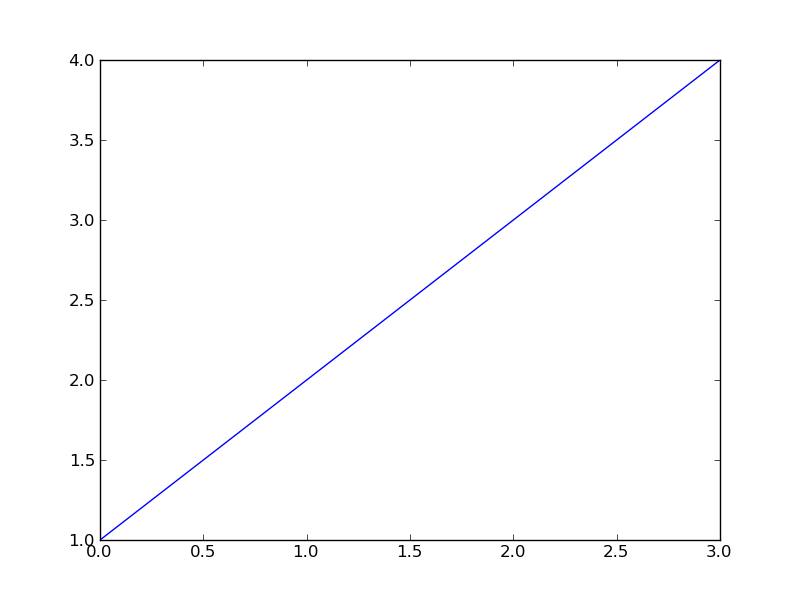
\includegraphics[width=\columnwidth]{figure1.png}}
\caption{This is the caption.:code:\DUroletitlereference{chunk of code} inside of it. \DUrole{label}{egfig}}
\end{figure}\begin{figure*}[]\noindent\makebox[\textwidth][c]{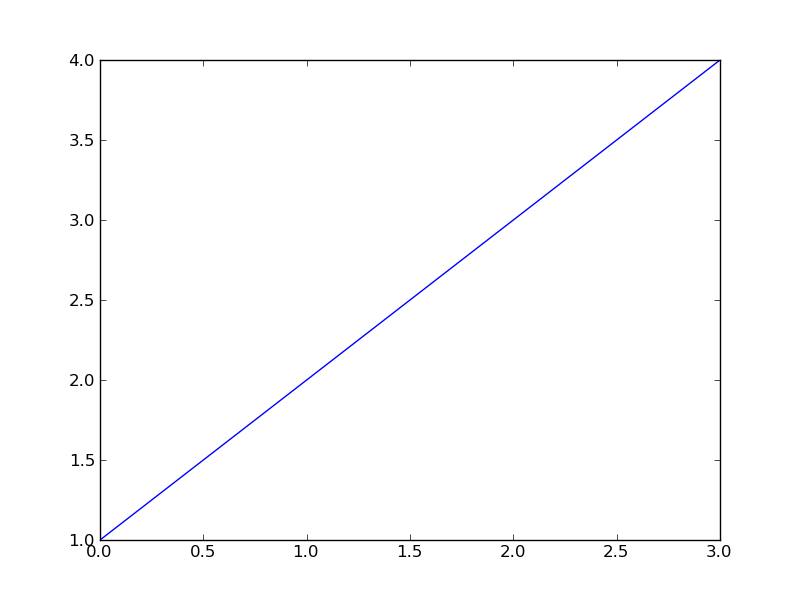
\includegraphics[width=\columnwidth]{figure1.png}}
\caption{This is a wide figure, specified by adding \textquotedbl{}w\textquotedbl{} to the figclass.  It is also
center aligned, by setting the align keyword (can be left, right or center).
This caption also has \texttt{\DUrole{code}{chunk of code}}.}
\end{figure*}\begin{figure}[bht]\noindent\makebox[\columnwidth][c]{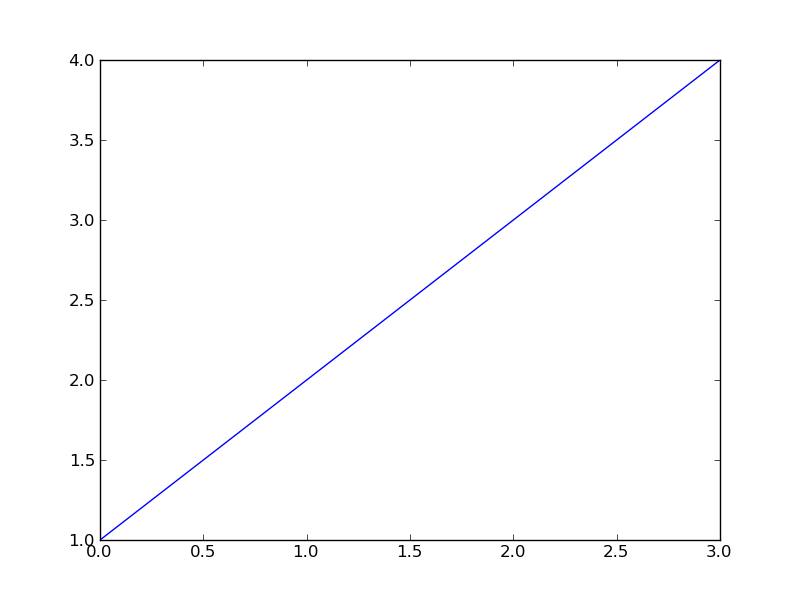
\includegraphics[scale=0.20]{figure1.png}}
\caption{This is the caption on a smaller figure that will be placed by default at the
bottom of the page, and failing that it will be placed inline or at the top.
Note that for now, scale is relative to a completely arbitrary original
reference size which might be the original size of your image - you probably
have to play with it.  \DUrole{label}{egfig2}}
\end{figure}

As you can see in Figures \DUrole{ref}{egfig} and \DUrole{ref}{egfig2}, this is how you reference auto-numbered
figures.\begin{table}
\setlength{\DUtablewidth}{\tablewidth}
\begin{longtable*}[c]{p{0.156\DUtablewidth}p{0.203\DUtablewidth}}
\toprule
\textbf{%
Material} & \textbf{%
Units} \\
\midrule
\endfirsthead

Stone & 
3 \\

Water & 
12 \\

Cement & 
$\alpha$ \\
\bottomrule
\end{longtable*}
\caption{This is the caption for the materials table. \DUrole{label}{mtable}}\end{table}

We show the different quantities of materials required in Table
\DUrole{ref}{mtable}.
% The statement below shows how to adjust the width of a table.

\setlength{\tablewidth}{0.8\linewidth}
\begin{table*}
\setlength{\DUtablewidth}{\tablewidth}
\begin{longtable*}[c]{p{0.110\DUtablewidth}p{0.063\DUtablewidth}p{0.086\DUtablewidth}p{0.086\DUtablewidth}p{0.086\DUtablewidth}p{0.086\DUtablewidth}p{0.110\DUtablewidth}}
\toprule

This & 
is & 
a & 
very & 
very & 
wide & 
table \\
\bottomrule
\end{longtable*}
\caption{This is the caption for the wide table.}\end{table*}

Unfortunately, restructuredtext can be picky about tables, so if it simply
won't work try raw LaTeX:
\begin{table*}

  \begin{longtable*}{|l|r|r|r|}
  \hline
  \multirow{2}{*}{Projection} & \multicolumn{3}{c|}{Area in square miles}\tabularnewline
  \cline{2-4}
   & Large Horizontal Area & Large Vertical Area & Smaller Square Area\tabularnewline
  \hline
  Albers Equal Area  & 7,498.7 & 10,847.3 & 35.8\tabularnewline
  \hline
  Web Mercator & 13,410.0 & 18,271.4 & 63.0\tabularnewline
  \hline
  Difference & 5,911.3 & 7,424.1 & 27.2\tabularnewline
  \hline
  Percent Difference & 44\% & 41\% & 43\%\tabularnewline
  \hline
  \end{longtable*}

  \caption{Area Comparisons \DUrole{label}{quanitities-table}}

\end{table*}


Perhaps we want to end off with a quote by Lao Tse\DUfootnotemark{id6}{id7}{3}:\begin{quotation}
\begin{quote}

\emph{Muddy water, let stand, becomes clear.}\end{quote}
\end{quotation}%
\DUfootnotetext{id7}{id6}{3}{$\mathrm{e^{-i\pi}}$}

% Customised LaTeX packages

% -------------------------

% Please avoid using this feature, unless agreed upon with the

% proceedings editors.

% ::

% .. latex::

% :usepackage: somepackage

% Some custom LaTeX source here.

\begin{thebibliography}{Atr03}
\bibitem[Atr03]{Atr03}{

P. Atreides. \emph{How to catch a sandworm},
Transactions on Terraforming, 21(3):261-300, August 2003.}
\end{thebibliography}

\end{document}
